\chapter{Validation par simulation MATLAB : PID, identification et commande MVC}

\section*{Introduction}

Ce chapitre présente la mise en œuvre pratique des concepts théoriques expliqués dans le chapitre précédent. L'objectif est d'étudier et de comparer les performances de deux stratégies de commande : la commande PID classique et la commande par réseau de neurones, appliquées à des systèmes de natures fondamentalement différentes.

La commande PID, dont la loi de commande repose sur la connaissance implicite du modèle du système, est dans un premier temps appliquée à des systèmes \textbf{linéaires invariants} (SLI). Le cas classique étudié ici est le système du second ordre de fonction de transfert :
\begin{equation}
	H(s) \;=\;
	\frac{K\,\omega_n^2}{s^2 + 2\,\xi\,\omega_n\,s + \omega_n^2}
	\label{eq:sys_second_ordre}
\end{equation}
où $K$ est le gain statique, $\xi$ le coefficient d'amortissement et $\omega_n$ la pulsation naturelle. Pour ces systèmes, le régulateur PID permet d'assurer un bon suivi de consigne sous réserve d'un réglage approprié des paramètres $(K_p, K_i, K_d)$.

Cependant, le régulateur PID atteint ses limites face aux systèmes \textbf{non linéaires}, pour lesquels aucune fonction de transfert ne peut représenter fidèlement le comportement. C'est pourquoi, dans un second temps, nous recourons à la commande neuronale par MLP, capable d'apprendre implicitement la dynamique du système à partir de données d'entrée-sortie.

Le système considéré est un \textbf{système non linéaire à mémoire}, dont la dynamique est la suivante :
\begin{equation}
	y(k) \;=\;
	-\,\frac{0{,}8\;a(k)\;\bigl[u(k-1)\bigr]^2}
	{1 + \bigl[u(k-1)\bigr]^2}
	+ 0{,}033\;y(k-1)
	+ 0{,}5\;u(k-1)
	\label{eq:sys_nl2_y}
\end{equation}
avec :
\[
a(k) \;=\; y(k-2)
\label{eq:sys_nl2_a}
\]
La non-linéarité est portée par le terme $\dfrac{a(k)\,[u(k-1)]^2}{1+[u(k-1)]^2}$, dont la saturation en entrée et la dépendance aux retards $y(k-1)$, $y(k-2)$ et $u(k-1)$ rendent toute linéarisation locale inadaptée.

L'ensemble de ces simulations est réalisé sous \textsc{Matlab} et permet d'évaluer, pour chaque stratégie de commande, les critères de performance obtenus.

%=====================================================
\section{Simulation et analyse de la commande PID numérique}
%=====================================================

Cette section présente l'étude comparative des performances du correcteur PID appliqué à un modèle de second ordre, représentatif de la dynamique de systèmes physiques réels.

%-----------------------------------------------------
\subsection{Commande PID d'un système du second ordre}
%-----------------------------------------------------

\subsubsection{Présentation du système et discrétisation}

On considère un système du second ordre de fonction de transfert :
\begin{equation}
	H(s) \;=\; \frac{K_s\,\omega_0^2}
	{s^2 + 2\,\xi\,\omega_0\,s + \omega_0^2}
	\label{eq:sys_2ordre}
\end{equation}
avec les paramètres numériques suivants :

\begin{table}[H]
	\centering
	\caption{Paramètres du système du second ordre.}
	\renewcommand{\arraystretch}{1.3}
	\begin{tabular}{lccc}
		\hline
		\textbf{Paramètre} & Gain $K_s$ & Pulsation propre $\omega_0$
		& Amortissement $\xi$ \\
		\hline
		\textbf{Valeur}    & $5$        & $20\,\text{rad/s}$ & $0{,}5$ \\
		\hline
	\end{tabular}
	\label{tab:params_sys_2ordre}
\end{table}

Le coefficient d'amortissement $\xi = 0{,}5 < 1$ caractérise donc un régime \textbf{sous-amorti} du système : la réponse indicielle en boucle ouverte présente un dépassement avant d'atteindre le régime permanent, comme l'illustre la figure~\ref{fig:reponse-indicielle}.

\begin{figure}[H]
	\centering
	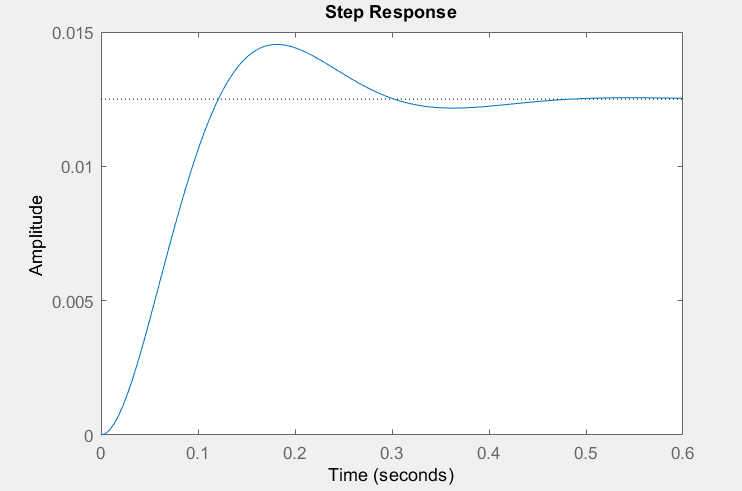
\includegraphics[width=0.7\linewidth]{figures/Reponse indicielle}
	\caption{Réponse indicielle du système du second ordre en boucle ouverte.}
	\label{fig:reponse-indicielle}
\end{figure}

La période d'échantillonnage est choisie égale à $T_e = 0{,}36\,\text{s}$. La discrétisation par ZOH donne :
\begin{equation}
	H(z) \;=\; \frac{b_1\,z^{-1} + b_2\,z^{-2}}
	{1 + a_1\,z^{-1} + a_2\,z^{-2}}
	\label{eq:sys_2ordre_z}
\end{equation}
dont l'équation récurrente est :
\begin{equation}
	y(k) \;=\; -a_1\,y(k-1) - a_2\,y(k-2)
	+ b_1\,u(k-1) + b_2\,u(k-2)
	\label{eq:recurrente_2ordre}
\end{equation}

\subsubsection{Loi de commande PID discrète et calcul des coefficients}

La même loi incrémentale est appliquée. Les coefficients retenus sont $c_0 = 15$, $c_1 = 1$, $c_2 = 1$. En inversant les relations :
\[
K_d \;=\; c_2 \cdot T_e \;=\; 0{,}36, \qquad
K_p \;=\; -c_1 - \frac{2\,K_d}{T_e} \;=\; -3, \qquad
K_i \;=\; \frac{c_0 - K_p - K_d/T_e}{T_e} \;\approx\; 47{,}2
\]

\begin{table}[H]
	\centering
	\caption{Paramètres du correcteur PID discret pour le système du second ordre.}
	\renewcommand{\arraystretch}{1.3}
	\begin{tabular}{lccc}
		\hline
		\textbf{Coefficient discret} & $c_0$ & $c_1$ & $c_2$ \\
		\hline
		\textbf{Valeur}              & $15$  & $1$   & $1$   \\
		\textbf{Paramètre PID}       & $K_p = -3$ & $K_i \approx 47{,}2$
		& $K_d = 0{,}36$ \\
		\hline
	\end{tabular}
	\label{tab:params_pid_2ordre}
\end{table}

\subsubsection{Résultats de simulation et interprétation}

La simulation est conduite sur $N = 100$ échantillons avec le même signal de référence en échelon double que précédemment.

\begin{figure}[H]
	\centering
	\begin{subfigure}[t]{0.49\textwidth}
		\centering
		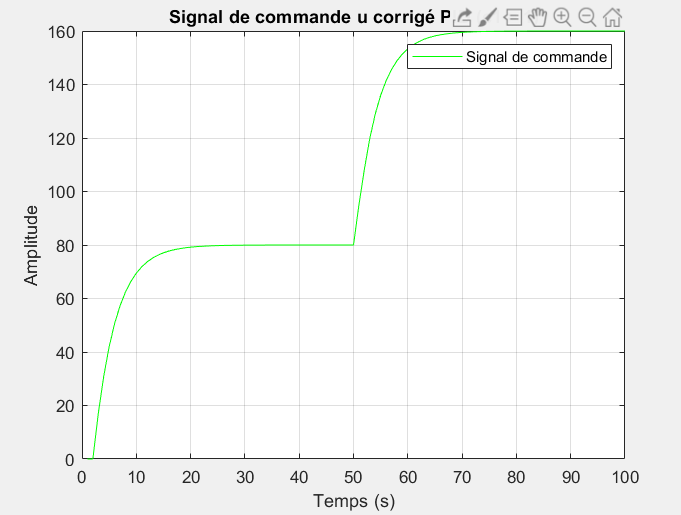
\includegraphics[width=\textwidth, height=7cm, keepaspectratio]
		{figures/Commande deuxieme ordre_PID}
		\caption{Signal de commande $u(k)$ généré par le correcteur PID.}
		\label{fig:commande_pid_2ordre}
	\end{subfigure}
	\hfill
	\begin{subfigure}[t]{0.49\textwidth}
		\centering
		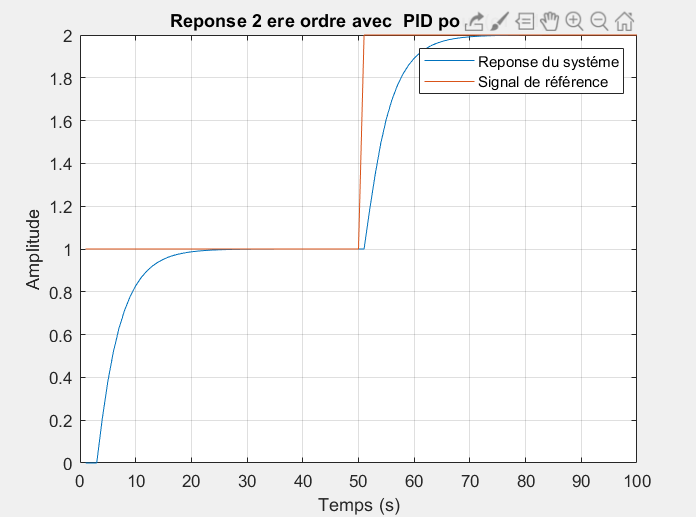
\includegraphics[width=\textwidth, height=7cm, keepaspectratio]
		{figures/Reponse du systeme de deuxieme ordre PID}
		\caption{Réponse $y(k)$ du système du second ordre régulé par PID.}
		\label{fig:reponse_pid_2ordre}
	\end{subfigure}
	\caption{Simulation de la commande PID appliquée au système du second ordre ($K_s = 5$, $\omega_0 = 20\,\text{rad/s}$, $\xi = 0{,}5$).}
	\label{fig:pid_2ordre}
\end{figure}

\paragraph{L'évolution du signal de commande $u(k)$}
\begin{itemize}[label=$\bullet$]
	
	\item La commande évolue de façon exponentielle croissante jusqu'à atteindre la valeur finale dans le premier régime et dans le deuxième régime imposé par la consigne.
	
\end{itemize}

\paragraph{Réponse du système $y(k)$}
\begin{itemize}[label=$\bullet$]
	
	\item Le système adopte bien la réponse d'un système du premier ordre, grâce à l'action du correcteur PID. Sa réponse suit bien la consigne sans erreur statique au régime permanent, aussi bien dans le premier que dans le deuxième régime imposé.
	
\end{itemize}

\paragraph{Bilan de la commande PID}
Les simulations confirment l'efficacité du régulateur PID discret pour les systèmes linéaires invariants. Cependant, le réglage manuel des coefficients $(c_0, c_1, c_2)$ suppose une connaissance implicite de la dynamique du système. Face à des systèmes non linéaires ou à modèle inconnu, cette approche devient inadaptée, ce qui motive le recours à la commande neuronale présentée dans la section suivante.

%=====================================================
\section{Identification par réseaux de neurones}
%=====================================================

\subsection{Objectif et démarche}

L'objectif de cette section est d'évaluer la capacité d'un réseau de neurones à \textbf{identifier} la dynamique de systèmes non linéaires à partir de leurs seules données d'entrée-sortie, sans connaissance préalable du modèle mathématique. Dans les deux cas, l'apprentissage est réalisé par l'\textbf{algorithme de descente de gradient par lots} (\textit{batch gradient descent}), dont la convergence est évaluée à travers le critère quadratique :
\[
C_r(p) \;=\; \sum_{k=3}^{N} \bigl(g(k) - y(k)\bigr)^2
\]

où $p$ désigne le numéro de l'époque (\textit{epoch}), c'est-à-dire le numéro du passage complet sur l'ensemble des données.

\textbf{Remarque :} la sommation sur le critère $C_r(p)$ commence à $k = 3$ car la sortie $y(k)$ du système dépend des échantillons aux instants $k-1$ et $k-2$. Le script Matlab commence par $k \geq 1$, on commence donc à $k = 3$ pour éviter les indices négatifs.

%-----------------------------------------------------
\subsection{Identification du système non linéaire à mémoire}
%-----------------------------------------------------

\subsubsection{Propriétés du système}

Le signal $y(k)$ est généré à partir d'une commande aléatoire $u(k) \in [-0{,}5,\; 0{,}5]$ selon l'équation récurrente :
\begin{equation}
	y(k) \;=\; -\frac{0{,}8\,y(k-2)\,[u(k-1)]^2}
	{1 + [u(k-1)]^2}
	+ 0{,}033\,y(k-1) + 0{,}5\,u(k-1)
	\label{eq:sys_memoire}
\end{equation}
Ce système présente deux niveaux de complexité : une \textbf{non-linéarité statique} (terme quadratique saturant) et une \textbf{dynamique à mémoire} (dépendance aux retards $k-1$ et $k-2$).

\subsubsection{Topologie du neurone d'identification}

Pour modéliser cette dynamique, le neurone utilise un vecteur d'entrée composé de la commande passée et du retour de sortie. La fonction d'activation choisie est la tangente hyperbolique ($\tanh$).

\begin{itemize}[label=$\bullet$]
	\item \textbf{Vecteur d'entrée :}
	$\mathbf{X}(k) = [-1,\; u(k-1),\; y(k-1)]^\top$
	\item \textbf{Vecteur des poids :}
	$\mathbf{W} = [w_0,\; w_1,\; w_2]^\top$
	\item \textbf{Sortie prédite :}
	$\hat{y}(k) = \tanh\!\bigl(-w_0 + w_1\,u(k-1)
	+ w_2\,y(k-1)\bigr)$
\end{itemize}

\paragraph{Choix du pas d'adaptation $\mu$.}
Le pas $\mu$ est l'hyperparamètre central de la descente de gradient. Sa valeur conditionne directement la vitesse et la stabilité de la convergence. La condition théorique de convergence impose :
\[
0 \;<\; \mu \;<\; \frac{2}{\lambda_{\max}}
\]
où $\lambda_{\max}$ est la plus grande valeur propre de la matrice de corrélation des entrées. En pratique, trois régimes sont observés :

\begin{table}[H]
	\centering
	\caption{Effet du pas d'adaptation $\mu$ sur la convergence.}
	\renewcommand{\arraystretch}{1.3}
	\begin{tabular}{lll}
		\hline
		\textbf{Valeur de $\mu$} & \textbf{Comportement}    & \textbf{Risque}        \\
		\hline
		$\mu = 0{,}001$          & Convergence très lente   & Arrêt prématuré        \\
		$\mu = 0{,}01$           & Convergence régulière    & Compromis optimal      \\
		$\mu = 0{,}1$            & Convergence rapide       & Oscillations possibles \\
		\hline
	\end{tabular}
	\label{tab:mu_convergence}
\end{table}

\subsubsection{Résultats et interprétation}

\begin{figure}[H]
	\centering
	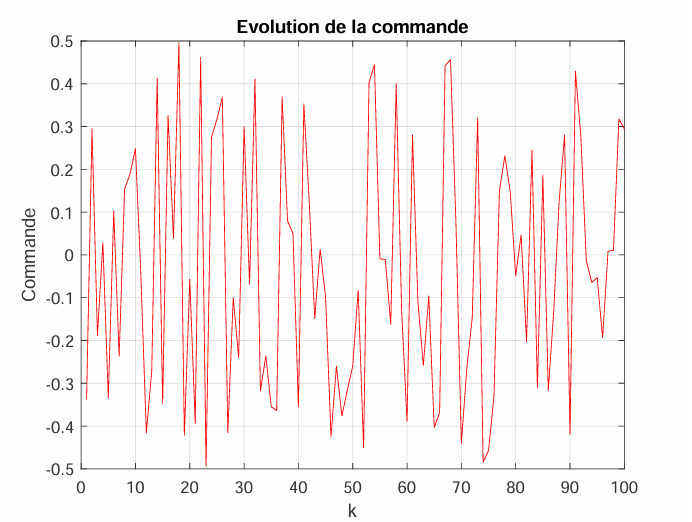
\includegraphics[width=0.8\linewidth]{figures/Commande_U_Rand}
	\caption{Évolution de la commande aléatoire $u(k) \in [-0{,}5,\; 0{,}5]$.}
	\label{fig:commandeurand}
\end{figure}

\begin{figure}[H]
	\centering
	\begin{subfigure}[t]{0.49\textwidth}
		\centering
		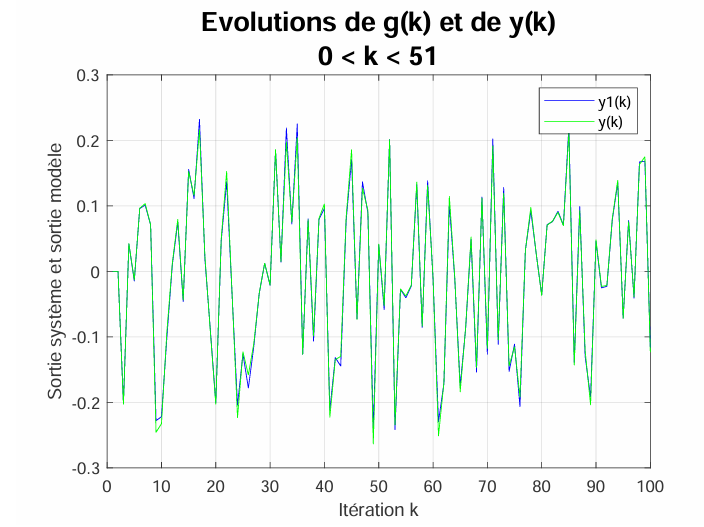
\includegraphics[width=\textwidth, height=6cm, keepaspectratio]
		{figures/Evolution}
		\caption{Évolution comparée de $y(k)$ et $\hat{y}(k)$.}
		\label{fig:evolution_y_id}
	\end{subfigure}
	\hfill
	\begin{subfigure}[t]{0.49\textwidth}
		\centering
		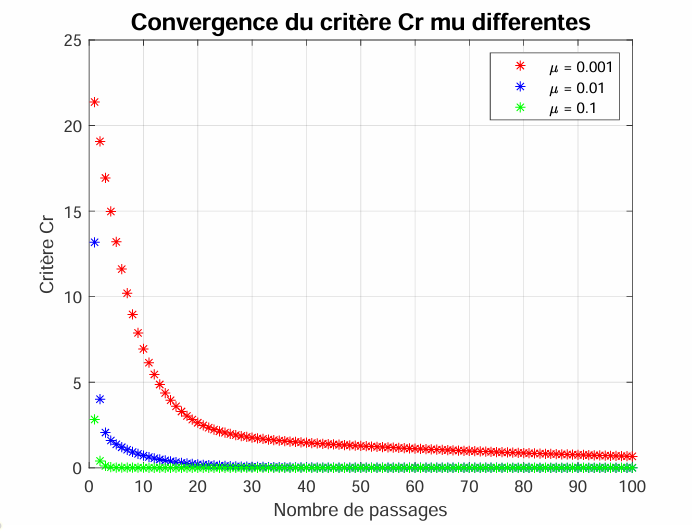
\includegraphics[width=\textwidth, height=6cm, keepaspectratio]
		{figures/Cr}
		\caption{Évolution du critère $C_r$ pour $\mu \in \{0{,}001,\; 0{,}01,\; 0{,}1\}$.}
		\label{fig:evolution_cr}
	\end{subfigure}
	\caption{Résultats de l'identification du système à mémoire.}
	\label{fig:resultats_memoire}
\end{figure}

\paragraph{Analyse de la convergence}
\begin{itemize}[label=$\bullet$]
	\item \textbf{$\mu = 0{,}001$} : La convergence du critère est extrêmement lente.
	\item \textbf{$\mu = 0{,}01$} : Décroissance régulière du critère $C_r$.
	\item \textbf{$\mu = 0{,}1$} : La convergence est la plus rapide.
\end{itemize}

\paragraph{Analyse du suivi}
Malgré la complexité de l'équation récurrente~\eqref{eq:sys_memoire}, le neurone parvient à suivre la dynamique du système. Les légers écarts observés s'expliquent par le fait que le modèle ne dispose que du retard $y(k-1)$ en entrée, alors que le système original dépend également de $y(k-2)$. La capacité de généralisation de la fonction $\tanh$ permet néanmoins de compenser partiellement cette information manquante.

\begin{table}[H]
	\centering
	\caption{Bilan comparatif de l'identification neuronale.}
	\renewcommand{\arraystretch}{1.3}
	\begin{tabular}{lcc}
		\hline
		\textbf{Critère}       & \textbf{Signal $g(k)$}
		& \textbf{Système à mémoire}    \\
		\hline
		Type de non-linéarité  & Statique multi-fréq.
		& Dynamique à retards            \\
		Entrées du neurone     & $g(k-1)$, $g(k-2)$
		& $u(k-1)$, $y(k-1)$            \\
		Convergence            & $p_{\max} \geq 50$
		& $\mu = 0{,}01$ optimal         \\
		Précision finale       & $C_r \approx 0$
		& Suivi satisfaisant             \\
		\hline
	\end{tabular}
	\label{tab:bilan_neuronal}
\end{table}

%=====================================================
\section{Commande par minimum de variance}
%=====================================================

Après avoir identifié le modèle neuronal du système, nous mettons en œuvre une stratégie de commande par minimum de variance (MV). L'objectif est de trouver la commande $u(k)$ permettant à la sortie $y(k)$ du système d'atteindre la consigne $y_c(k)$ en minimisant les effets du bruit $e(k)$. On cherche à déterminer, à chaque instant $k$, la commande $u(k)$ optimale capable de minimiser l'écart entre la sortie prédite et une consigne imposée $y_c(k)$.

\subsection{Critère de performance}

Pour éviter des variations trop brusques de la commande qui pourraient déstabiliser le système réel, nous utilisons un critère quadratique incluant une pénalisation sur l'effort de commande :
\begin{equation}
	J(u(k)) = [y_c(k+1) - \hat{y}(k+1)]^2 + \lambda [u(k) - u(k-1)]^2
	\label{eq:critere_mv}
\end{equation}
Où :
\begin{itemize}[label = $\bullet$]
	\item $y_c(k+1)$ est la consigne à l'instant suivant.
	\item $\hat{y}(k+1)$ est la prédiction du modèle neuronal.
	\item $\lambda$ est le facteur de pondération.
\end{itemize}

\subsection{Algorithme d'optimisation itérative}

Le modèle étant non linéaire (présence de la fonction $\tanh$), la commande optimale $u(k)$ ne peut être extraite analytiquement. Nous utilisons donc un algorithme de descente de gradient interne à chaque période d'échantillonnage, sur un nombre d'itérations $i_{max} = 10$ :

\paragraph{Correction d'erreur :}
Afin d'améliorer la précision du prédicteur, nous introduisons un terme correctif $\alpha$ (facteur d'apprentissage ou de recalage) qui prend en compte l'erreur résiduelle entre la sortie réelle $y(k)$ et la prédiction précédente $\hat{y}(k)$ :
\begin{equation}
	\hat{y}(k+1) = \tanh(v(k)) + \alpha \cdot (y(k) - \hat{y}(k))
\end{equation}

\paragraph{Mise à jour de la commande :}
Le gradient du critère par rapport à la commande $x$ (représentant $u(k)$) est calculé par :
\begin{equation}
	\frac{\partial J}{\partial x} = -2 \cdot (y_c(k+1) - \hat{y}(k+1)) \cdot \frac{\partial \hat{y}(k+1)}{\partial x} + 2\lambda(x - u(k-1))
\end{equation}
Avec $\frac{\partial \hat{y}(k+1)}{\partial x} = (1 - \tanh(v)^2) \cdot w_1$. La nouvelle valeur de la commande est ensuite mise à jour avec un pas $\mu = 0{,}2$ :
\begin{equation}
	u(k)_{new} = u(k)_{old} - \mu \frac{\partial J}{\partial x}
\end{equation}

\subsection{Résultats et analyse du suivi}

Le test a été effectué sur un profil de consigne en échelons ($0{,}3$, $0{,}6$ et $0{,}5$).

\begin{figure}[H]
	\centering
	\begin{subfigure}[t]{0.49\textwidth}
		\centering
		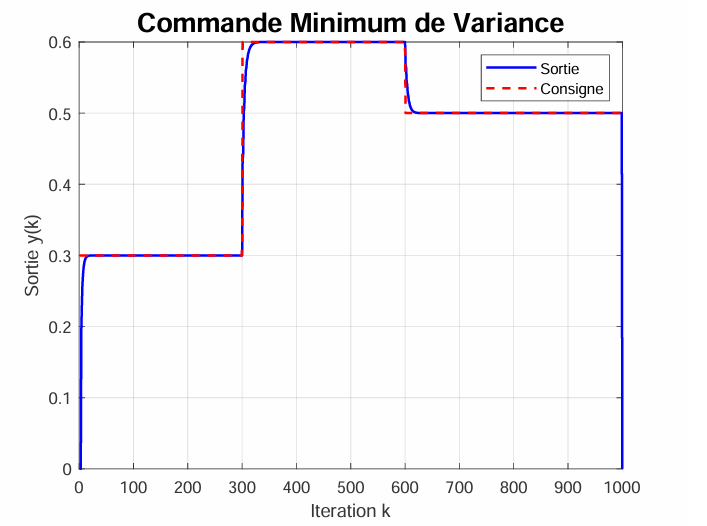
\includegraphics[width=\textwidth, height=6cm, keepaspectratio]
		{figures/Suiv_Consigne}
		\caption{Suivi de consigne par commande Minimum de Variance.}
		\label{fig:suivi_consigne_mv}
	\end{subfigure}
	\hfill
	\begin{subfigure}[t]{0.49\textwidth}
		\centering
		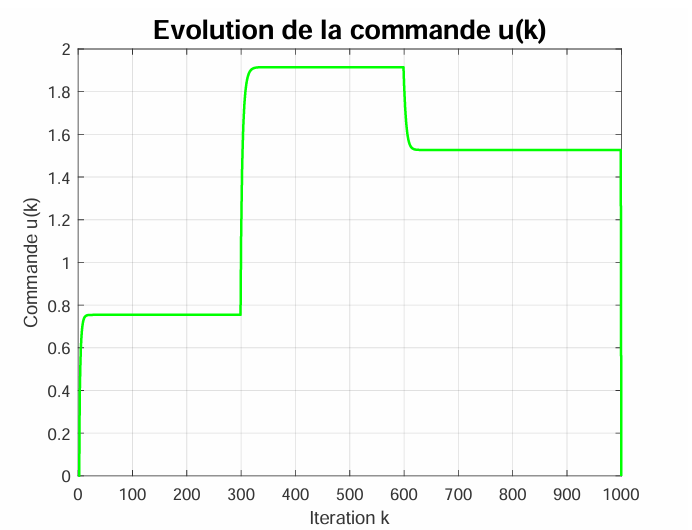
\includegraphics[width=\textwidth, height=6cm, keepaspectratio]
		{figures/Commande_MV_1}
		\caption{Commande par minimum de variance.}
		\label{fig:commande_mv}
	\end{subfigure}
	\caption{Résultats de la commande par minimum de variance.}
	\label{fig:resultats_mv}
\end{figure}

\paragraph{Interprétation :}
Comme illustré sur la Figure \ref{fig:suivi_consigne_mv}, la sortie $y(k)$ rejoint rapidement la consigne $y_c(k)$ malgré la forte non-linéarité du système réel. L'évolution de la commande $u(k)$ montre des pics d'accélération sans dépassement, suivis d'une stabilisation rapide vers le régime permanent. La valeur de $\lambda$ très faible permet une réactivité élevée, tandis que l'algorithme itératif assure que le modèle neuronal est "inversé" correctement à chaque pas, garantissant ainsi un minimum de variance de l'erreur de suivi.

\begin{figure}[H]
	\centering
	\begin{subfigure}[t]{0.49\textwidth}
		\centering
		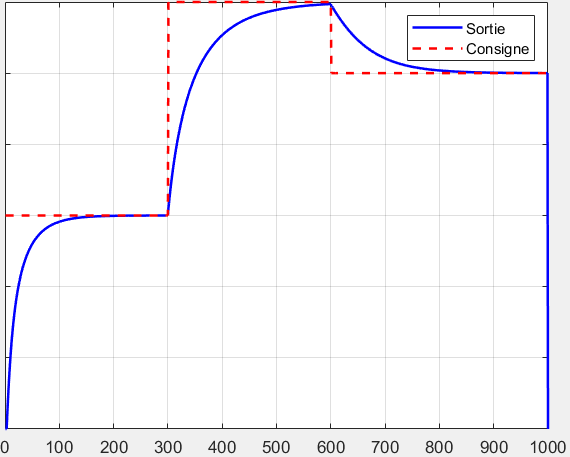
\includegraphics[width=\textwidth, height=6cm, keepaspectratio]{figures/R_MV_Lambda_4}
		\caption{Suivi de consigne pour les grandes valeurs de $\lambda$ ($\lambda = 4$).}
		\label{fig:rmvlambda4}
	\end{subfigure}
	\hfill
	\begin{subfigure}[t]{0.49\textwidth}
		\centering
		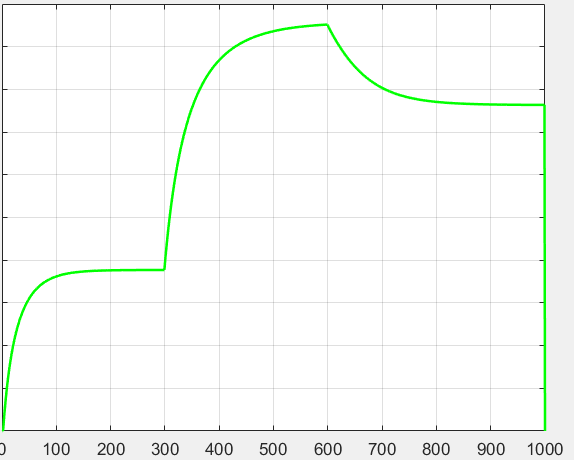
\includegraphics[width=\textwidth, height=6cm, keepaspectratio]{figures/MV_Lambda_4}
		\caption{Évolution de la commande par minimum de variance pour $\lambda = 4$.}
		\label{fig:mvlambda4}
	\end{subfigure}
	\caption{Changement de la réactivité du système pour les grandes valeurs de régularisation sur la commande.}
	\label{fig:High_lambda}
\end{figure}

Dans la figure \ref{fig:High_lambda}, on observe qu'une forte régularisation sur la commande a influencé la rapidité du système et sa précision. En effet, d'après la figure \ref{fig:mvlambda4}, la commande n'a pas encore atteint le régime permanent pendant le premier et le deuxième changement de consigne, et la réponse du système est en grand retard par rapport à la consigne.

%=====================================================
\section*{Conclusion}
%=====================================================

Ce chapitre a présenté une étude comparative des deux stratégies de commande étudiées dans ce travail. La commande PID discrète, appliquée au système du second ordre, a démontré ses bonnes performances sur les systèmes linéaires invariants : erreur statique nulle, absence de dépassement et suivi correct de consigne variable. La principale limite réside dans la nécessité d'un réglage manuel des paramètres, qui suppose une connaissance de la dynamique du système.

Face aux systèmes non linéaires, la commande neuronale par descente de gradient a montré sa capacité à identifier implicitement la dynamique à partir des seules données d'entrée-sortie. Les résultats obtenus valident l'efficacité de l'algorithme de rétropropagation.

Ces résultats de simulation constituent le fondement théorique nécessaire à l'implémentation expérimentale présentée dans le chapitre suivant, qui portera sur l'application de ces méthodes à la régulation thermique réelle de l'enceinte.